The recognition of gestures is based on measured acceleration values. These
values depend, as it was already depicted in section \ref{sect:dataModel}, on
the orientation of the smartphone. The mathematical relation of the measured
acceleration values and the smartphone's orientation will be derived in this
chapter. At first, the impact the smartphone being rotated along one of its axes
is investigated in isolation. Afterwards, the results are combined and the final
equation for each of the acceleration values is set up.
\label{sect:mathBasics}

\subsection{Terminology of the possible Rotations}

\begin{figure}
\centering
\captionsetup{justification=centering}
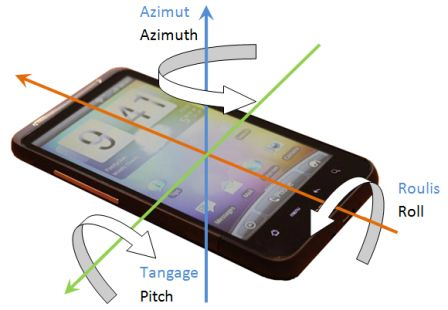
\includegraphics[width=0.75\textwidth]{res/mathstuff/rotations.jpg}
\caption{Possibilities of rotating a Smartphone, see \cite{objectifNux}}
\label{fig:DataModel}
\end{figure}

There exist three different possible rotations that are measured by the magnetic field sensor:

\begin{itemize}
\item{
\textbf{Pitch} \newline
The angle of a rotation around the x-axis is called pitch. In the following
equations, $\alpha$ will be used to describe the value of pitch that is
retrieved from the magnetic field sensor.
}
\item{
\textbf{Roll} \newline
The angle of a rotation around the y-axis is called roll. In the following
equations, $\beta$ will be used to describe the value of roll that is retrieved
from the magnetic field sensor.
}
\item{
\textbf{Azimuth} \newline
The angle of a rotation around the z-axis is called azimuth. In the following
equations, $\gamma$ will be used to describe the value of azimuth that is
retrieved from the magnetic field sensor.
}
\end{itemize}


\subsection{Acceleration depending on Pitch}
The current section investigates the effect of a rotation around the
smartphone's x-axis on the measured acceleration values. Figures
\ref{fig:yPitch} and \ref{fig:zPitch} show how accelerations in the direction of
x and of z respectively might be decomposed into the different
acceleration vectors that are parallel to the smartphone's axes. The 
magnitudes of these vectors are measured by the smartphone's acceleration
sensor.

\begin{figure}[htb]
    \centering
    \begin{minipage}{0.5\textwidth}
        \centering
        \captionsetup{justification=centering}
        
  \begin{tikzpicture}
	\newcommand{\cosAngle}{0.866}
	\newcommand{\sinAngle}{0.5}
	\newcommand{\sideLength}{2}
	\newcommand{\mobileLength}{4}
	\newcommand{\hlh}{\mobileLength/2}
	\newcommand{\mobileThickness}{0.25}
    	
	\coordinate (origo) at (0,0);
    	\coordinate (point_on_x) at (2,0);

	\coordinate (end_a_y) at (-\hlh - \sideLength*\cosAngle,-1);
	

   	\begin{scope}[rotate=30]
		\coordinate (end_a_y_mobile) at (-\hlh-\cosAngle*\sideLength,0);
		\coordinate (begin_a_y) at (-\hlh, 0);

    		\fill[gray] ($ (origo) + (-\hlh,-\mobileThickness/2) $) rectangle ($ (origo) + (\hlh,\mobileThickness/2) $);
		\draw[dashed, black] (-\hlh,0)--(\hlh,0);
		\coordinate (rotated) at (\hlh,0);
		 \draw[thick,orange,->] (begin_a_y)  -- (end_a_y_mobile) node (y_mobile)
		 [orange,below] {$a_{y, mobile}$}; \begin{scope}[rotate=-30]
			\draw[very thick,red,->] (-\hlh*\cosAngle,-1)  -- (end_a_y) node (y_real)
			[red,above] {$a_y$}; 
			\draw[thick,blue,->](end_a_y_mobile)
						--
						(-\hlh - \sideLength*\cosAngle,-1) node (z_mobile) [blue, left] {$a_{z,
						mobile}$};
		\end{scope}
	\end{scope}	
    	% draw axes
    	\fill[black] (origo) circle (0.05);
    	\draw[thick,orange,->] (origo) -- ++(2,0) node[black,right] {$y$};
    	\draw[thick,blue,->] (origo) -- ++(0,-2) node (mary) [black,below] {$z$};
   	\draw[thick] ($ (origo) + (-1,0) $) -- ($ (origo) + (1,0) $);

	% angle axes
	\tkzMarkAngle[fill= orange,size=1.2cm,opacity=.4](point_on_x,origo,rotated)
    	\pic [draw, ->, "$\alpha$", angle eccentricity=1.5] {angle =
    	point_on_x--origo--rotated};

	% angle vectors
	\tkzMarkAngle[fill=
	orange,size=1.2cm,opacity=.4](end_a_y,begin_a_y,end_a_y_mobile) \pic [draw, ->,
	"$\alpha$", angle eccentricity=1.5] {angle = end_a_y--begin_a_y--end_a_y_mobile};
  \end{tikzpicture}
        \caption{$a_y$ depending on Pitch}
        \label{fig:yPitch}
    \end{minipage}% <- sonst wird hier ein Leerzeichen eingef�gt
    \hfill
    \begin{minipage}{0.5\textwidth}
        \centering
			\begin{align} 
				a_{z, handy} &= \tan(\alpha) \cdot {a_{y, handy}}\\
				a_y &= \frac{a_{y, handy}}{\cos(\alpha)}
			\end{align}
    \end{minipage}
\end{figure}

\begin{figure}[htb]
    \centering
    \begin{minipage}{0.5\textwidth}
        \centering
        \captionsetup{justification=centering}
          \begin{tikzpicture}
	\newcommand{\cosAngle}{0.866}
	\newcommand{\sinAngle}{0.5}
	\newcommand{\sideLength}{2}
	\newcommand{\handyLength}{4}
	\newcommand{\hlh}{\handyLength/2}
	\newcommand{\handyThickness}{0.25}
    	
	\coordinate (origo) at (0,0);
    	\coordinate (point_on_x) at (2,0);
	
	\begin{scope}[rotate=30]
		\coordinate (begin_a_z) at (-\hlh, 0);
	\end{scope}	

	\coordinate (end_a_y) at ($(begin_a_z)+(0,-\sideLength)$);
	\draw[thick,red,->] (begin_a_z) -- (end_a_y) node (y_real) [red,above left]
	{$a_z$}; 
	\begin{scope}[rotate=30]
		%\coordinate (end_a_z_handy) at ($(begin_a_z)+(0,-\sideLength)$);
		\coordinate (end_a_z_handy) at ($(begin_a_z)+(0,-\cosAngle*\sideLength)$);
	\end{scope}	
	\draw[thick,blue,->] (begin_a_z) -- (end_a_z_handy) node (z_handy) [blue,above
	right] {$a_{z, handy}$};

	\draw[thick,orange,->] (end_a_z_handy)  -- (end_a_y) node (y_handy)
	[orange,below right] {$a_{y, handy}$};

   	\begin{scope}[rotate=30]
		\coordinate (end_a_y_handy) at (-\hlh-\sideLength,0);
		%\coordinate (begin_a_z) at (-\hlh, 0);

    		\fill[gray] ($ (origo) + (-\hlh,-\handyThickness/2) $) rectangle ($ (origo) + (\hlh,\handyThickness/2) $);
		\draw[dashed, black] (-\hlh,0)--(\hlh,0);
		\coordinate (rotated) at (\hlh,0);
	\end{scope}	
    	% draw axes
    	\fill[black] (origo) circle (0.05);
    	\draw[thick,orange,->] (origo) -- ++(2,0) node[black,right] {$y$};
    	\draw[thick,blue,->] (origo) -- ++(0,-1.5) node (mary) [black,below] {$z$};
   	\draw[thick] ($ (origo) + (-1,0) $) -- ($ (origo) + (1,0) $);

	% angle axes
	\tkzMarkAngle[fill= orange,size=1.2cm,opacity=.4](point_on_x,origo,rotated)
    	\pic [draw, ->, "$\alpha$", angle eccentricity=1.5] {angle = point_on_x--origo--rotated};

	% angle vectors
	\tkzMarkAngle[fill=
	orange,size=1.2cm,opacity=.4](end_a_y,begin_a_z,end_a_z_handy) \pic [draw, ->,
	"$\alpha$", angle eccentricity=1.5] {angle = end_a_y--begin_a_z--end_a_z_handy};
  \end{tikzpicture}
        \caption{$a_z$ depending on Pitch}
        \label{fig:zPitch}
    \end{minipage}% <- sonst wird hier ein Leerzeichen eingef�gt
    \hfill
    \begin{minipage}{0.5\textwidth}
        \centering
			\begin{align} 
				a_{y, handy} &= \tan(\alpha) \cdot a_{z, handy}\\ 
				a_z &= \frac{a_{z, handy}}{\cos(\alpha)}
			\end{align}
    \end{minipage}
\end{figure}

\FloatBarrier
\subsection{Acceleration depending on Roll}
A rotation around a certain axis affects the measured acceleration values of the
axes that are parallel to axis of rotation. Therefore, if the smartphone is
rotated around its y-axis, the accelerations in the direction of x and z have to
be investigated. The composition of the acceleration vectors can be retrieved
from the figures \ref{fig:xRoll} and \ref{fig:zRoll}.

\begin{figure}[htb]
    \centering
    \begin{minipage}{0.5\textwidth}
        \centering
        \captionsetup{justification=centering}
          \begin{tikzpicture}
	\newcommand{\cosAngle}{0.866}
	\newcommand{\sinAngle}{0.5}
	\newcommand{\sideLength}{2}
	\newcommand{\handyLength}{4}
	\newcommand{\hlh}{\handyLength/2}
	\newcommand{\handyThickness}{0.75}
    	
	\coordinate (origo) at (0,0);
    	\coordinate (point_on_x) at (2,0);

	\coordinate (end_a_y) at (-\hlh - \sideLength*\cosAngle,-1);
	

   	\begin{scope}[rotate=30]
		\coordinate (end_a_y_handy) at (-\hlh-\cosAngle*\sideLength,0);
		\coordinate (begin_a_y) at (-\hlh, 0);

    		\fill[gray] ($ (origo) + (-\hlh,-\handyThickness/2) $) rectangle ($ (origo) + (\hlh,\handyThickness/2) $);
		\draw[dashed, black] (-\hlh,0)--(\hlh,0);
		\coordinate (rotated) at (\hlh,0);
		 \draw[thick,green,->] (begin_a_y)  -- (end_a_y_handy) node (y_handy)
		 [green,below] {$a_{x, handy}$}; \begin{scope}[rotate=-30]
			\draw[very thick,red,->] (-\hlh*\cosAngle,-1)  -- (end_a_y) node (y_real)
			[red,above] {$a_x$}; 
			\draw[thick,blue,->](end_a_y_handy)
						--
						(-\hlh - \sideLength*\cosAngle,-1) node (z_handy) [blue, left] {$a_{z,
						handy}$};
		\end{scope}
	\end{scope}	
    	% draw axes
    	\fill[black] (origo) circle (0.05);
    	\draw[thick,green,->] (origo) -- ++(2,0) node[black,right] {$x$};
    	\draw[thick,blue,->] (origo) -- ++(0,-2) node (mary) [black,below] {$z$};
   	\draw[thick] ($ (origo) + (-1,0) $) -- ($ (origo) + (1,0) $);

	% angle axes
	\tkzMarkAngle[fill= green,size=1.2cm,opacity=.4](point_on_x,origo,rotated)
    	\pic [draw, ->, "$\beta$", angle eccentricity=1.5] {angle =
    	point_on_x--origo--rotated};

	% angle vectors
	\tkzMarkAngle[fill=
	green,size=1.2cm,opacity=.4](end_a_y,begin_a_y,end_a_y_handy) \pic [draw, ->,
	"$\beta$", angle eccentricity=1.5] {angle = end_a_y--begin_a_y--end_a_y_handy};
  \end{tikzpicture}
        \caption{$a_x$ depending on Roll}
        \label{fig:xRoll}
    \end{minipage}% <- sonst wird hier ein Leerzeichen eingef�gt
    \hfill
    \begin{minipage}{0.5\textwidth}
        \centering
			\begin{align} 
				a_{z, handy} &= \tan(\beta) \cdot {a_{x, handy}}\\
				a_x &= \frac{a_{x, handy}}{\cos(\beta)}
			\end{align}
    \end{minipage}
\end{figure}

\begin{figure}[htb]
    \centering
    \begin{minipage}{0.5\textwidth}
        \centering
        \captionsetup{justification=centering}
          \begin{tikzpicture}
	\newcommand{\cosAngle}{0.866}
	\newcommand{\sinAngle}{0.5}
	\newcommand{\sideLength}{2}
	\newcommand{\mobileLength}{4}
	\newcommand{\hlh}{\mobileLength/2}
	\newcommand{\mobileThickness}{0.75}
    	
	\coordinate (origo) at (0,0);
    	\coordinate (point_on_x) at (2,0);
	
	\begin{scope}[rotate=30]
		\coordinate (begin_a_z) at (-\hlh, 0);
	\end{scope}	

	\coordinate (end_a_y) at ($(begin_a_z)+(0,-\sideLength)$);
	\draw[thick,red,->] (begin_a_z) -- (end_a_y) node (y_real) [red,above left]
	{$a_z$}; 
	\begin{scope}[rotate=30]
		%\coordinate (end_a_z_mobile) at ($(begin_a_z)+(0,-\sideLength)$);
		\coordinate (end_a_z_mobile) at ($(begin_a_z)+(0,-\cosAngle*\sideLength)$);
	\end{scope}	
	\draw[thick,blue,->] (begin_a_z) -- (end_a_z_mobile) node (z_mobile) [blue,above
	right] {$a_{z, mobile}$};

	\draw[thick,green,->] (end_a_z_mobile)  -- (end_a_y) node (y_mobile)
	[green,below right] {$a_{x, mobile}$};

   	\begin{scope}[rotate=30]
		\coordinate (end_a_y_mobile) at (-\hlh-\sideLength,0);
		%\coordinate (begin_a_z) at (-\hlh, 0);

    		\fill[gray] ($ (origo) + (-\hlh,-\mobileThickness/2) $) rectangle ($ (origo) + (\hlh,\mobileThickness/2) $);
		\draw[dashed, black] (-\hlh,0)--(\hlh,0);
		\coordinate (rotated) at (\hlh,0);
	\end{scope}	
    	% draw axes
    	\fill[black] (origo) circle (0.05);
    	\draw[thick,green,->] (origo) -- ++(2,0) node[black,right] {$x$};
    	\draw[thick,blue,->] (origo) -- ++(0,-1.5) node (mary) [black,below] {$z$};
   	\draw[thick] ($ (origo) + (-1,0) $) -- ($ (origo) + (1,0) $);

	% angle axes
	\tkzMarkAngle[fill= green,size=1.2cm,opacity=.4](point_on_x,origo,rotated)
    	\pic [draw, ->, "$\beta$", angle eccentricity=1.5] {angle = point_on_x--origo--rotated};

	% angle vectors
	\tkzMarkAngle[fill= green,size=1.2cm,opacity=.4](end_a_y,begin_a_z,end_a_z_mobile)
    	\pic [draw, ->, "$\beta$", angle eccentricity=1.5] {angle = end_a_y--begin_a_z--end_a_z_mobile};
  \end{tikzpicture}

        \caption{$a_z$ depending on Roll}
        \label{fig:zRoll}
    \end{minipage}% <- sonst wird hier ein Leerzeichen eingef�gt
    \hfill
    \begin{minipage}{0.5\textwidth}
        \centering
			\begin{align} 
				a_{x, handy} &= \tan(\beta) \cdot a_{z, handy}\\ 
				a_z &= \frac{a_{z, handy}}{\cos(\beta)}
			\end{align}
    \end{minipage}
\end{figure}

\FloatBarrier
\subsection{Acceleration depending on Azimuth}
The last rotation that is examined is the one around the z-axis. This rotation
affects the measured acceleration values in the direction of x and y. The
vector-decomposition is depicted in the figures \ref{fig:xAzimuth} and
\ref{fig:yAzimuth}.

\begin{figure}[htb]
    \centering
    \begin{minipage}{0.5\textwidth}
        \centering
        \captionsetup{justification=centering}
          \begin{tikzpicture}
	\newcommand{\cosAngle}{0.866}
	\newcommand{\sinAngle}{0.5}
	\newcommand{\sideLength}{2}
	\newcommand{\handyLength}{4}
	\newcommand{\hlh}{\handyLength/2}
	\newcommand{\handyWidth}{2}
	\newcommand{\hwh}{\handyWidth/2}
	\newcommand{\padding}{0.25}

	\begin{scope}[rotate=120]
		\draw[rounded corners] (-\hlh,-\hwh) rectangle (\hlh,\hwh);
		\draw[rounded corners] (-\hlh+\padding,-\hwh+\padding) rectangle (\hlh-\padding,\hwh-\padding);
		\draw[dashed, black] (-\hlh,0)--(\hlh,0);
		\draw[dashed, black] (0,-\hwh)--(0,\hwh);
		\coordinate (begin_a_x) at (0, -\hwh);
	\end{scope}
	
	\coordinate (end_a_x) at ($(begin_a_x)+(\sideLength,0)$);
	\draw[very thick,red,->] (begin_a_x)  -- (end_a_x) node (x_real) [red,below] {$a_x$}; 

	\coordinate (end_a_x_handy) at ($(begin_a_x)+(\cosAngle*\cosAngle*\sideLength,\sinAngle*\cosAngle*\sideLength)$);
	\draw[thick,green,->] (begin_a_x)  -- (end_a_x_handy) node (x_handy) [green,above] {$a_{x, handy}$};
	
	\draw[thick,orange,->] (end_a_x_handy) -- (end_a_x) node (y_handy) [orange,above right] {$a_{y, handy}$};

	\begin{scope}[rotate=30]
		\coordinate (rotated) at (0,2);
	\end{scope}
    	
	\coordinate (origo) at (0,0);
    	\coordinate (point_on_z) at (0,2);

	\coordinate (end_a_y) at (-\hlh - \sideLength*\cosAngle,-1);

    	% draw axes
    	\fill[black] (origo) circle (0.05);
    	\draw[thick,green,->] (origo) -- ++(2,0) node[black,right] {$x$};
    	\draw[thick,orange,->] (origo) -- ++(0,3) node (mary) [black,below left] {$y$};
   	\draw[thick] ($ (origo) + (-1,0) $) -- ($ (origo) + (1,0) $);

	% angle axes
	\tkzMarkAngle[fill= blue,size=1.2cm,opacity=.4](point_on_z,origo,rotated)
    	\pic [draw, ->, "$\gamma$", angle eccentricity=1.5] {angle =
    	point_on_z--origo--rotated};

	% angle vectors
	\tkzMarkAngle[fill=
	blue,size=1.2cm,opacity=.4](end_a_x,begin_a_x,end_a_x_handy) \pic [draw, ->,
	"$\gamma$", angle eccentricity=1.5] {angle = end_a_x--begin_a_x--end_a_x_handy};
  \end{tikzpicture}
        \caption{$a_x$ depending on Azimuth}
        \label{fig:xAzimuth}
    \end{minipage}% <- sonst wird hier ein Leerzeichen eingef�gt
    \hfill
    \begin{minipage}{0.5\textwidth}
        \centering
			\begin{align} 
				a_{y, handy} &= \tan(\gamma) \cdot {a_{x, handy}}\\
				a_x &= \frac{a_{x, handy}}{\cos(\gamma)}
			\end{align}
    \end{minipage}
\end{figure}

\begin{figure}[htb]
    \centering
    \begin{minipage}{0.5\textwidth}
        \centering
        \captionsetup{justification=centering}
          \begin{tikzpicture}
	\newcommand{\cosAngle}{0.866}
	\newcommand{\sinAngle}{0.5}
	\newcommand{\sideLength}{2}
	\newcommand{\mobileLength}{4}
	\newcommand{\hlh}{\mobileLength/2}
	\newcommand{\mobileWidth}{2}
	\newcommand{\hwh}{\mobileWidth/2}
	\newcommand{\padding}{0.25}

	\begin{scope}[rotate=120]
		\draw[rounded corners] (-\hlh,-\hwh) rectangle (\hlh,\hwh);
		\draw[rounded corners] (-\hlh+\padding,-\hwh+\padding) rectangle (\hlh-\padding,\hwh-\padding);
		\draw[dashed, black] (-\hlh,0)--(\hlh,0);
		\draw[dashed, black] (0,-\hwh)--(0,\hwh);
		\coordinate (begin_a_y) at (\hlh, 0);
	\end{scope}
	
	\coordinate (end_a_y) at ($(begin_a_y)+(0, \sideLength)$);
	\draw[very thick,red,->] (begin_a_y)  -- (end_a_y) node (x_real) [red,below right] {$a_y$}; 

	\coordinate (end_a_y_mobile) at ($(begin_a_y)+(-\sinAngle*\cosAngle*\sideLength,\cosAngle*\cosAngle*\sideLength)$);
	\draw[thick,orange,->] (begin_a_y)  -- (end_a_y_mobile) node (y_mobile) [orange,above left] {$a_{y, mobile}$};
	
	\draw[thick,green,->] (end_a_y_mobile) -- (end_a_y) node (y_mobile) [green,above] {$a_{x, mobile}$};

	\begin{scope}[rotate=30]
		\coordinate (rotated) at (0,2);
	\end{scope}
    	
	\coordinate (origo) at (0,0);
    	\coordinate (point_on_z) at (0,2);

    	% draw axes
    	\fill[black] (origo) circle (0.05);
    	\draw[thick,green,->] (origo) -- ++(2,0) node[black,right] {$x$};
    	\draw[thick,orange,->] (origo) -- ++(0,3) node (mary) [black,below left] {$y$};
   	\draw[thick] ($ (origo) + (-1,0) $) -- ($ (origo) + (1,0) $);

	% angle axes
	\tkzMarkAngle[fill= blue,size=1.2cm,opacity=.4](point_on_z,origo,rotated)
    	\pic [draw, ->, "$\gamma$", angle eccentricity=1.5] {angle =
    	point_on_z--origo--rotated};

	% angle vectors
	\tkzMarkAngle[fill=	blue,size=1.2cm,opacity=.4](end_a_y,begin_a_y,end_a_y_mobile) 
	\pic [draw, ->,"$\gamma$", angle eccentricity=1.5] {angle = end_a_y--begin_a_y--end_a_y_mobile};
  \end{tikzpicture}
        \caption{$a_y$ depending on Azimuth}
        \label{fig:yAzimuth}
    \end{minipage}% <- sonst wird hier ein Leerzeichen eingef�gt
    \hfill
    \begin{minipage}{0.5\textwidth}
        \centering
			\begin{align} 
				a_{x, handy} &= \tan(\gamma) \cdot a_{y, handy}\\ 
				a_y &= \frac{a_{y, handy}}{\cos(\gamma)}
			\end{align}
    \end{minipage}
\end{figure}

\subsection{Final Equations for the Acceleration Values}
After the acceleration values have been examined depending on each rotation
value in isolation, the results are combined together in this section.

\subsubsection{Final Equation: X-Acceleration }
As it has been shown in the equations $(1.6)$ and $(1.10)$, the acceleration in
the direction of x depends on the values of roll and azimuth. Combining these
two equations leads to the following equation:

\begin{equation}
a_x = \frac{a_{x, handy}}{\cos(\beta) \cdot \cos(\gamma)}
\end{equation}

\noindent The measured value of $a_{x,handy}$ is affected in two cases:
\begin{itemize}
\item{if the handy is accelerated in the direction of z and the value of roll is
not equal to 0}
\item{if the handy is accelerated in the direction of y and the value of azimuth is not equal to 0}
\end{itemize}
These affectations are defined by the equations $(1.7)$ and $(1.11)$. Taking
these equations into account leads to the following, final equation:

\begin{equation}
a_x = \frac{a_{x, handy} \cdot (1 - \tan(\beta) \cdot a_{z, handy}
- \tan(\gamma) \cdot a_{y, handy})}{\cos(\beta) \cdot \cos(\gamma)}
\end{equation}

\subsubsection{Final Equation: Y-Acceleration }
The equations $(1.2)$ and $(1.12)$ show the dependency of an acceleration in the
direction of y on the values of pitch and azimuth. If these equations
are put together, the result is given by:

\begin{equation}
a_y = \frac{a_{y, handy}}{\cos(\alpha) \cdot \cos(\gamma)}
\end{equation}

\noindent The measured value of $a_{y,handy}$ is affected in two cases:
\begin{itemize}
\item{if the handy is accelerated in the direction of z and the value of pitch is not equal to 0}
\item{if the handy is accelerated in the direction of x and the value of azimuth is not equal to 0}
\end{itemize}
Therefore, the equations $(1.3)$ and $(1.9)$ have to be included in the
calculations.
This leads to the following, final equation:

\begin{equation}
a_y = \frac{a_{y, handy} \cdot (1 - \tan(\alpha) \cdot a_{z, handy}
- \tan(\gamma) \cdot a_{x, handy})}{\cos(\alpha) \cdot \cos(\gamma)}
\end{equation}

\subsubsection{Final Equation: Z-Acceleration }
The basic equation for the acceleration in the direction of z is retrieved by assembling the equations $(1.4)$ and $(1.8)$ that define the accelerations dependency on the values of roll and pitch respectively. 
\begin{equation}
a_z = \frac{a_{z, handy}}{\cos(\alpha) \cdot \cos(\beta)}
\end{equation}

\noindent The measured value of $a_{z,handy}$ is affected in two cases:
\begin{itemize}
\item{if the handy is accelerated in the direction of y and the value of pitch is not equal to 0}
\item{if the handy is accelerated in the direction of x and the value of roll is not equal to 0}
\end{itemize}
If these cases (see equations $(1.1)$ and $(1.5)$) are considered, the final
equation is given by:
\begin{equation}
a_z = \frac{a_{z, handy} \cdot (1 - \tan(\alpha) \cdot a_{y, handy}
- \tan(\beta) \cdot a_{x, handy})}{\cos(\alpha) \cdot \cos(\beta)}
\end{equation}
